% $Id: circuit.tex 7840 2020-06-09 17:04:06Z mskala $

%
% MSK 009 circuit explanation
% Copyright (C) 2018  Matthew Skala
%
% This program is free software: you can redistribute it and/or modify
% it under the terms of the GNU General Public License as published by
% the Free Software Foundation, version 3.
%
% This program is distributed in the hope that it will be useful,
% but WITHOUT ANY WARRANTY; without even the implied warranty of
% MERCHANTABILITY or FITNESS FOR A PARTICULAR PURPOSE.  See the
% GNU General Public License for more details.
%
% You should have received a copy of the GNU General Public License
% along with this program.  If not, see <http://www.gnu.org/licenses/>.
%
% Matthew Skala
% https://northcoastsynthesis.com/
% mskala@northcoastsynthesis.com
%

\chapter{Circuit explanation}

The MSK~009 Coiler VCF is a conventional two-pole state-variable design with
a twist, or rather a couple of coils.  The general theory of similar filters
with capacitor-based integrators can be found in any textbook on active
filters and I do not propose to go through it in great detail here; instead,
I will give an intuitive description of the operating principle, using no
more than elementary calculus, and then note some details specific to the
Coiler.

%%%%%%%%%%%%%%%%%%%%%%%%%%%%%%%%%%%%%%%%%%%%%%%%%%%%%%%%%%%%%%%%%%%%%%%%

\section{Two-pole state-variable intuition}

The expression $\sin f\!x$ describes a sine wave of frequency $f$ radians per
unit of time $x$.  Let's take the integral of that.

\begin{equation*}
  \int \sin f\!x \, dx = - \frac{1}{f} \cos f\!x
\end{equation*}

The integral of a sine wave is just another sine wave at the same frequency,
shifted by 90$^\circ$, and scaled by the inverse of the frequency.  If we
take another integral, it gets shifted another 90$^\circ$ for a total of
180$^\circ$.

\begin{equation*}
  \iint \sin f\!x \, dx = - \frac{1}{f^2} \sin f\!x
\end{equation*}

The frequency response of a voltage integrator circuit, plotted on a Bode
plot, is just a downward slope of 6dB/octave or 20dB/decade.  Note that it
hits unity gain (0dB) at normalized frequency 1, where the 1/$f$ terms in
the integrals become unity.

\nopagebreak
{\centering\includegraphics[width=0.9\linewidth]{intbode.eps}\par}

Now, consider the frequency response of a two-pole Butterworth high-pass
filter.  There is some curvature in the graph around the cutoff, but
significantly above the cutoff frequency, it is flat (0dB/octave), and
significantly below the cutoff, it rises at 12dB/octave.

\nopagebreak
{\centering\includegraphics[width=0.9\linewidth]{hpbode.eps}\par}

What happens if we take a circuit with a high-pass response, and integrate
its output?  The integrator response is falling at 6dB/octave.  When applied
to the 12dB/octave rise below the cutoff, that leaves a 6dB/octave rise. 
When applied to the flat response above cutoff, the integrator changes the
response to falling at 6dB/octave.  Overall, we have a band-pass response
with 6dB/octave slopes on both sides.

\nopagebreak
{\centering\includegraphics[width=0.9\linewidth]{bpbode.eps}\par}

It may not show clearly at this scale, but the peak of the band-pass
response does not reach 0dB but only $-$3dB, due to the curvature of the
high-pass response in the vicinity of the cutoff frequency.

Now suppose we attach another integrator to the circuit.  The lower slope,
rising at 6dB/octave, is cancelled out, and the upper slope, falling at
6dB/octave, is steepened to 12dB/octave.  The result is a two-pole low-pass
response.

\nopagebreak
{\centering\includegraphics[width=0.9\linewidth]{lpbode.eps}\par}

So a low-pass response is just the integral of a band-pass response, which
is the integral of a high-pass.
These relations provide the start of a recipe for a multimode filter:  just
start with a high-pass response and attach two integrators.  Then we have a
filter with three outputs, high-, band-, and low-pass.  But where will
the high-pass response come from?

Consider the sum of the low-pass and high-pass responses.  Remember that
taking two integrals of a sine wave entails a 180$^\circ$ phase shift; a
voltage inversion.  At the cutoff frequency, the low-pass and high-pass
responses will be equal, but with opposite phase, so they cancel out to
zero.  Above or below the cutoff frequency, one or the other of the low- and
high-pass responses will be near 0dB while the other is much lower, and the
sum will be close to 0dB.  So the sum of the low- and high-pass responses is
a notch response.

\nopagebreak
{\centering\includegraphics[width=0.9\linewidth]{ntbode.eps}\par}

Adding in the band-pass response as well can fill in that notch; but because
the peak of the bandpass is 3dB down, it's necessary to put in a bit of
gain; specifically, boosting the voltage by $\sqrt{2}$, which doubles the
power (3dB gain).  With that modification, the sum of the three filter
outputs recovers the input (at least, if we ignore phase).

\begin{equation*}
   \textit{IN} = \textit{HP} + \sqrt{2}\textit{BP} + \textit{LP}
\end{equation*}

We can solve for the high-pass response and find that it is the sum of
(possibly scaled and inverted) copies of the input, band-pass, and low-pass
responses.  And that is the missing piece for the multimode filter.  The
filter core will consist of two integrators in series, driven by a mixer
that combines the input and the two integrator outputs, with scaling and
inversion.

\vspace{0.5\baselineskip}
{\centering\input{coretopo.tex}\par}

There are many variations on the basic two-pole state-variable filter.  Some
provide multiple inputs instead of multiple outputs, by mixing in the
different inputs at different points along the chain of integrators; and the
details of the scaling and inversion vary depending on the desired phase
relationships among the different responses.  In the Coiler in particular,
the mixer that creates the high-pass output inverts all three of its inputs
because that makes for a more convenient op amp circuit, and the voltage
gain on the band-pass feedback path is 2 at minimum resonance instead of
$\sqrt{2}$.

Note that everything in the theoretical description is scaled to the
frequency at which the integrators have unity gain.  If we add some gain or
attenuation at each integrator, the same at both of them, then we shift that
frequency without changing anything else; and so the cutoff frequency of the
filter changes.

%%%%%%%%%%%%%%%%%%%%%%%%%%%%%%%%%%%%%%%%%%%%%%%%%%%%%%%%%%%%%%%%%%%%%%%%

\section{Integrators}

The two-pole state-variable topology provides a framework for generating
many filter designs just by swapping in different integrator, mixer, and VCA
circuits.  There are many such designs on the market and most of them
distinguish themselves from others by using different VCAs; no VCA design
gives perfect voltage multiplication, especially in situations like
overdrive, and the differences in the VCAs' imperfections are supposed to
give different sounds.  The MSK~009 instead makes its main innovation in the
integrator circuit.

Here is the topology of a standard capacitor-based voltage integrator. 
Bearing in mind that the op amp negative input is a virtual ground, the
current through the resistor is directly proportional to the input voltage. 
Then the same current must flow through the capacitor (given the effectively
infinite input impedance of the op amp), and the voltage across the
capacitor is (by nature of a capacitor) the time integral of the current. 
Voltage out for the circuit is negative time integral of voltage in, scaled
by component values.

\vspace{0.5\baselineskip}
{\centering\input{capint.tex}\par}

The capacitor-based integrator goes from voltage input to voltage output,
with a 90$^\circ$ phase shift corresponding to integration, by internally
using a current in phase with the input.  But we can also design a similar
circuit that will use a current in phase with the output, as seen below.

\vspace{0.5\baselineskip}
{\centering\input{indint.tex}\par}

The current through the inductor is, by nature of an inductor, the time
integral of the voltage across the inductor.  Then the currents must balance
at the op amp negative input, so the same current flows through the
resistor, which converts it back to a voltage.  With ideal components, this
inductor-based voltage integrator is exactly equivalent to the capacitor
version.

But we do not have ideal components, especially not in the case of
inductors.  Small to medium capacitors are capable of approaching ideal
behaviour at audio frequencies, but inductors seldom come close, especially
not if they are of practical physical size and cost.  In particular, the
EPCOS ferrite bobbin inductors used in the Coiler VCF behave very much as
the following circuit made from ideal components would behave.

\vspace{0.5\baselineskip}
{\centering\input{equivcirc.tex}\par}

This equivalent circuit was found by a combination of measuring
real-life samples of the components, and fitting simulation results to the
curves in the data sheet.

When one of these non-ideal inductors is balanced against a plain resistor
in the inductive op amp integrator circuit, the behaviour depends on the
frequency.  At very high frequencies (far above audio), the 10pF capacitance
dominates.  The inductor behaves more like a capacitor, and the circuit is
more like a differentiator than an integrator.  At sufficiently low
frequencies, the inductance and capacitance are not significant and the
coil's behaviour is mostly controlled by its 90$\Omega$ resistance.  Then
the integrator circuit behaves like a plain inverting amplifier.  With the
component values used in the Coiler VCF, the point at which the inductors
start becoming more like resistors is at frequencies below about 1kHz; well
into the audio range.

So to balance the component that is like an inductor at higher frequencies
and like a resistor at lower frequencies, we will use something that is like
a resistor at higher frequencies and like a capacitor at lower frequencies,
namely a series circuit of a resistor and a near-ideal capacitor.  Over the
audio spectrum, the integrator shifts smoothly between capacitor-based
integration (resistor on input, capacitor in feedback loop) and
inductor-based integration (inductor on input, resistor in feedback loop).

\begin{figure*}
\centering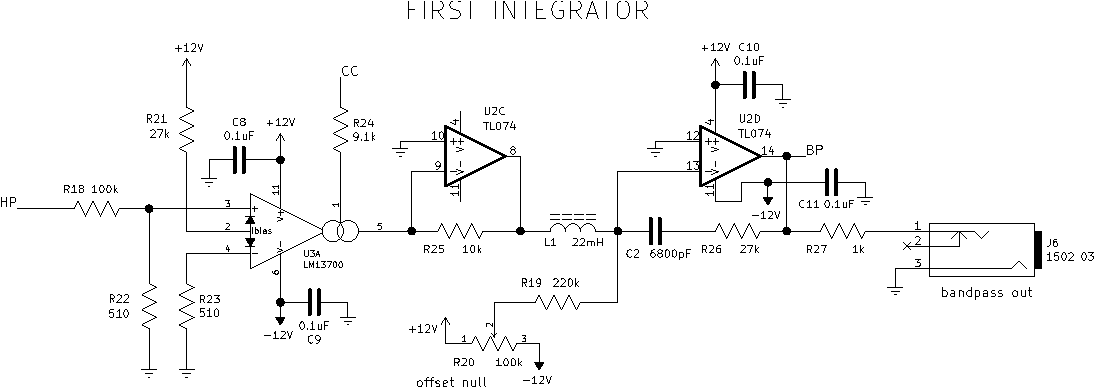
\includegraphics[width=\linewidth]{integrator.pdf}\par
\caption{One integrator in the filter core.}\label{fig:integrator}
\end{figure*}

See Figure~\ref{fig:integrator}.  The component L1 is labelled a 22mH
inductor, but bear in mind that because of the non-ideal behaviour of
real-life components, it only provides a near-pure inductance over a limited
range of frequencies.  At the bottom of the audio range, it is more like a
resistor.  The coil's capacitance can be ignored for most of this
discussion; that only comes into play at frequencies that should never be
present in this circuit.  The coil is at the input to the op amp U2D, whose
feedback loop contains a 6800pF capacitor and 27k$\Omega$ resistor.  At high
audio frequencies, when the inductor is really providing inductance, the
capacitor has low impedance and the feedback loop looks like a resistor;
then we have the inductor input, resistor feedback style of op amp
integrator.  At low frequencies, when the inductor looks more like a
resistor, the capacitor will have significant impedance and the circuit
functions as the resistor input, capacitor feedback style of op amp
integrator.

The resistance and capacitance values were chosen by simulation and
prototyping to give phase response as flat as possible.  However, this
response is not completely flat, not least because the model of the coil's
behaviour over frequency is only approximate.  As frequency varies over the
audio range, the phase response of the integrators, and therefore the
overall sound of the filter, will vary.

The other components in Figure~\ref{fig:integrator} are basically all
support for the integrator components L1, C2, R26, and U2A.  Immediately
before the coil, the op amp U2C and feedback resistor R25 function to
convert the current from the OTA into a voltage.  This section is needed
because the OTA, U3A, produces its output signal as a \emph{current} level
instead of a voltage.  Traditional capacitor-based integrators actually take
current input anyway, and use an input resistor to convert voltage to
current; when using such an integrator with an OTA, it is usual to leave out
the input resistor and run the OTA directly into the op amp's virtual
ground.  Keeping the OTA output at a fixed voltage helps mimize distortion. 
But becaus the Coiler's coils require real voltage input, not current, it's
necessary to convert the current to a voltage, and U2C and its feedback
resistor do that while allowing the OTA output to stay at 0V.

Immediately before the current to voltage converter comes the operational
transconductance amplifier U3A, with its support components.  This is the
variable-gain element used for tuning the filter.  It is a fairly
conventional design.  Note the linearizing diode current supplied by R21. 
This part is often left out of LM13700-based designs, but I like to include
it both because it improves distortion performance and because it makes the
gain of the amplifier more predictable, requiring less trimming.  The gain
of the amplifier is linearly controlled by a control current (labelled
``CC'' on the diagram) from the exponential converter to be described later. 
The 9.1k$\Omega$ resistor on that input helps both with keeping the gain of
the two integrators the same, and with limiting the control current to a
safe level.  The exponential converter is not capable of driving its output
voltage above 0V, so the maximum possible current through R24 is about
1.2mA, not enough to damage the LM13700.

\begin{figure*}
\centering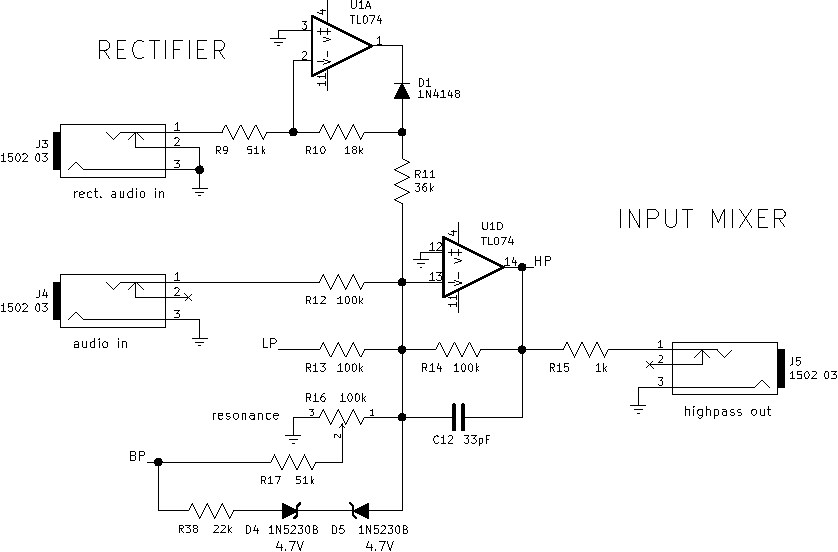
\includegraphics[scale=0.8]{input.pdf}\par
\caption{Input mixer and rectifier.}\label{fig:input}
\end{figure*}

The offset null trimmer R20, with its scale-setting resistor R19, helps to
compensate for input offsets in the op amps and OTAs (most significantly,
the OTAs).  There are seven IC amplifiers in the large feedback loop: one in
the input mixer and three in each of two integrators.  In principle, every
one of those amplifiers has an input offset, and trimming all of them would
require seven adjustments.  That is too many adjustments to be practical in
a commercial module.\footnote{I learned my lesson with the Leapfrog, which
has 13 trimmers.} Instead of trimming every single amplifier, there is one
trimmer on each integrator, and the idea is to average them out.  The exact
consequences of adding or subtracting an offset at this point in the circuit
are complicated; I used simulation to determine that R20 primarily affects
the externally visible offset on the HP and LP outputs, and R30 primarily
the BP and LP.  Not having precise trimming of the OTA offsets leads to a
more than trivial amount of control feedthrough, but I'm treating that as
just part of the unique sound of this module.  When the control signal is
coming from an envelope, some envelope feedthrough into audio may help
listeners perceive the envelope as ``snappy.''

The second integrator has just the same circuit as the first, and works the
same way.

%%%%%%%%%%%%%%%%%%%%%%%%%%%%%%%%%%%%%%%%%%%%%%%%%%%%%%%%%%%%%%%%%%%%%%%%

\section{Input mixer and rectifier}

The input mixer and rectifier sections are shown in Figure~\ref{fig:input}. 
The input mixer is straightforward: it is a standard inverting op-amp
summer, with inputs from the module input J4 and the low-pass and band-ass
integrator outputs.  The capacitor C12 is for stability at high frequencies;
since the capacitance of the coils can make the integrators stop being
integrators and switch over to doing differentiation once the frequency gets
high enough, there is the danger that the entire module could go into
parasitic oscillation at ultrasonic frequencies should there be enough
feedback around the loop at such frequencies.  The op amps themselves have
limited frequency range, but maybe not limited enough; the 33pF capacitor
kills the gain in the ultrasonic range and makes sure parasitic oscillation
will be impossible.

The feedback pass from the band-pass output is responsible for the
``resonance'' control and (deliberate) oscillation of the module.  Note the
pin numbers on the panel pot R16: when this knob is turned to its
user-visible ``minimum'' (full counterclockwise), the gain on the BP
feedback path is actually \emph{maximized} at about 2.  This feedback path
inhibits oscillation.  Increasing resonance reduces the gain on it,
ultimately as far as zero, at which point the module should oscillate
reliably.

If the only feedback is through the low-pass feedback path, then the
oscillations will build steadily until they drive the amplifiers into
clipping.  The output amplitude in that case is somewhat unpredictable
(because it depends on internal offsets we can only partially trim) and is
usually more than desired ($\pm$5V being a good target for maximum output in
Eurorack).  The clipping components R38, D4, and D5 help keep it under
control.  When oscillation reaches about $\pm$5V, the diodes start to
conduct, increasing the gain on the feedback path and inhibiting further
increase in the oscillation amplitude.  This specific placement of the
diodes (on the BP path, feeding into the op amp virtual ground) was chosen
largely by trial and error; I tried putting limiting circuits at several
other points but found they had the most reliable and pleasant-sounding
effects here.

The rectifier section, shown again below, is an unusual one.  Note that
unlike most op-amp precision full-wave rectifiers, this uses only one op amp
and one diode.  It's a near variation of one I have seen attributed to
``Tompkins, W.J., and J.G.  Webster (eds.), \textit{Interfacing Sensors to
the IBM PC.} Prentice-Hall, 1988'' but I have not actually read that
reference.

\vspace{0.5\baselineskip}
{\centering\input{fwrect.tex}\par}

Suppose the input voltage is positive.  In order to keep its negative input
at 0V, the op amp U1A must draw the same current through R10 that flows through
R9, and that means the voltage at the diode anode is $-18/51$ times the
input voltage.  Bearing in mind that the input mixer's summing node is kept
at 0V with a 100k$\Omega$ input impedance set by R14, the feedback resistor
on U1D, the gain from the diode anode to the input mixer's output (module HP
output) is $-100/36$, and that combined with the rectifier's $-18/51$ gain
is unity, to within component tolerances.

But suppose the input voltage is negative.  Nothing can drive the U1A
negative input to zero.  The only current sources available are the virtual
ground at the U1D negative input, which can only bring U1A's negative input
\textit{halfway} to zero through the resistor network; and the output of
U1A, which is on the far side of a reverse-biased diode.  Then the U1A
negative input remains below the positive input of 0V, U1A output heads for
the positive rail, but will have no effect, and the input voltage has a
straight shot through the series combination of R9, R10, and R11 (totalling
105k$\Omega$) into the 100k$\Omega$ \emph{inverting} impedance of the
mixer's summing node.  Gain from the rectifier input to the mixer's output
is close to \emph{negative} unity.

On positive input the gain is positive unity, and on negative input the gain
is negative unity.  Positive and negative input voltages both will translate
to positive output voltages; this is a full-wave rectifier.

The full-wave rectifier certainly isn't perfect.  There will be some
difference in gain between the positive and negative half-cycles due to the
use of standard components close to, rather than exactly, the right ratios. 
The op amp is being used with a large differential input range, driven into
saturation on negative input, which is not ideal.  But note that because of
the voltage division involved its input cannot go below about $-$6V for the
rated $\pm$12V input range, and so the phase inversion problem with
FET-input op amps like the TL074 is not an issue here.  The biggest problem
with this one-diode, one-op-amp full-wave circuit is that it only works
correctly when driving a fixed input impedance.  That is the case here
because we have the well-behaved summing node of the input mixer to drive,
but the circuit would require some sort of buffering if it were providing a
rectified output directly to the outside world.  Actually, the story of this
circuit is that the rest of the module required seven op amps, they come in
packages of four, and I didn't want to leave one unused.  The single-op-amp
full-wave rectifier circuit nicely used up available resources while
providing a musically useful extra feature.

%%%%%%%%%%%%%%%%%%%%%%%%%%%%%%%%%%%%%%%%%%%%%%%%%%%%%%%%%%%%%%%%%%%%%%%%

\section{Exponential converter}

The exponential converter is shown in Figure~\ref{fig:expoconv}.  It's a
fairly conventional design, with partial temperature compensation.

\begin{figure}
\centering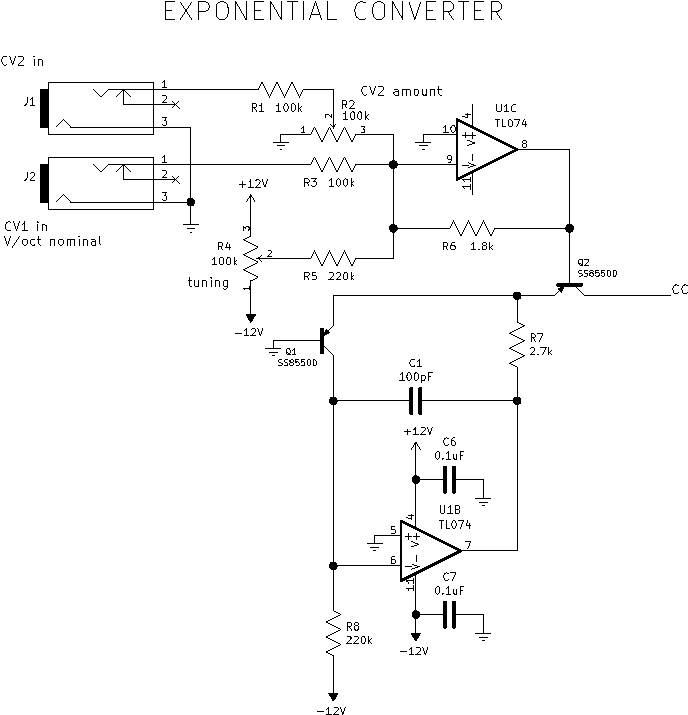
\includegraphics[width=\linewidth]{expoconv.pdf}\par
\caption{Exponential converter and control voltage
processor.}\label{fig:expoconv}
\end{figure}

The 1.8k$\Omega$ feedback resistor R6 sets the gain for U1C, on the CV1
input with its 100k$\Omega$ input resistor, to $-$18mV per volt of control
voltage input.  That is (approximately) the right amount to apply to the
base of a silicon transistor to double the collector current; so this gives
approximately 1V/octave response.  The CV2 and tuning-knob inputs are
straightforward, one having an attenuator and the other applying an offset
to the summing node of the front-end amplifier.

The second op amp, U1B, is the ``servo'' op amp for the temperature
compensation.  Its function is to keep the emitters of both transistors at
whatever voltage is necessary (probably around $+$0.7V) for such a
transistor to pass about 54$\mu$A when its base is at 0V.  The transistor
Q1, called the reference transistor, has its base permanently connected to
0V.  The current through this transistor is set by R8; constant current
because the high side of R8, and Q1's collector, are kept at 0V by op amp
feedback.  Then the op amp drives the emitters of the transistors as
necessary to maintain the right emitter-base voltage for that current level. 
This implies that if the control voltage from U1C happens to be zero, the
output current through Q2 to the ``CC'' connection (which feeds the
integrators) will also be 54$\mu$A.  For each additional volt on the V/oct
input, the control voltage applied to Q2 goes down 18mV, increasing the
emitter-base voltage by 18mV and doubling the current.

The reason for this complexity is that the desired emitter-base voltage for
a fixed current level can vary quite a bit with temperature.  If we used a
single transistor and a fixed assumption for the offset of the emitter-base
voltage, then the filter's frequency would change with any small temperature
variation, making tuning difficult.  Here, we make some effort to keep Q1
and Q2 at the same temperature and then any change in the required
emitter-base voltage for a fixed current will be detected and applied by the
servo op amp; the front-end op amp is only controlling the \emph{difference}
between the emitter-base voltages of Q1 and Q2.  This takes care of the main
temperature effect on tuning.

There is another temperature effect in the fact that the ``18mV'' quantity
representing how much differential voltage to apply for a doubling of
current, is itself temperature-dependent.  In the Coiler, there is no effort
made to compensate that voltage.  There are enough other inaccuracies and
unpredictable things in the design that it seems not to be worthwhile; users
requiring precise tracking will be using other filters, such as the MSK~007
Leapfrog.  But when this kind of exponential converter is used in other
applications, it is common practice to apply temperature compensation in the
front-end amplifier as well, often by replacing the feedback resistor with a
carefully chosen temperature-sensitive resistor or network.

Two other components worth mentioning in this section are C1 and R7, both of
which are intended to keep the op amp U1B stable.  Q1 has a lot of voltage
gain between its emitter and collector.  The current through the transistor,
and therefore the voltage at the collector given the current-to-voltage
characteristic of R8, is an exponential function of the emitter-base
voltage.  If we connected the emitter directly to the output of U1B, then
U1B would be in negative feedback with significant voltage gain around the
feedback loop, and that is likely to push it into parasitic oscillation.  Op
amps in general are not rated for stability with feedback loop gain greater
than unity.  So the resistor R7 is included to cut down the gain around the
loop.  With that resistance in series with the emitter-base drop, it
takes a much larger voltage change on the op amp output to produce a
significant change in current.  The capacitor C1 also serves to improve
stability by putting in a phase shift at high frequencies.  The servo op amp
should not respond faster than the highest modulation frequency of the
filter, so this capacitor prevents it from responding, and possibly
oscillating, in the ultrasonic range.
